\documentclass{scrartcl}
\usepackage{amsmath}
\usepackage{graphicx}
\usepackage{url}
\usepackage{listings}
\renewcommand{\lstlistingname}{Listing}
\title{Cubic Interpolation with Irregularly Spaced Points}
\subtitle{Version 1.0}
\author{R. Steven Turley}
\date{August 23, 2018}
\begin{document}
\maketitle
\tableofcontents

\section{Introduction}
This is the mathematics and some implementation details
behind a derivation of 1d cubic piece-wise continuous
interpolation with regularly and irregularly spaced points.
I will explore two ways to compute this cubics: splines and
Hermite polynomials. Both are continuous and have continuous
derivatives at the knots. Splines also have continuous second
derivatives.

\section{Cubic Splines}

I will use the article on splines for a regularly-spaced
grid in MathWorld\cite{mathworld} as a basis for my
derivations and generalizations.

Splines are piece-wise cubic polynomials which are continuous
and have continuous first and second derivatives. In each interval
it takes four coefficients to define a cubic polynomial. If there
are $n+1$ points, there are $n$ intervals requiring $4n$ coefficients
for the splines. Let the knots on the spline (the data points that
match exactly) be $(x_i,y_i)$. Let $Y_i(x)$ be the cubic polynomial for
the interval $i$ where $x_i\leq x\leq x_{i+1}$. Then the $4n-4$ conditions
for matching the points and having continuous first and second derivatives
are for $2\leq n \leq n$
\begin{align}
Y_{i-1}(x_i) &= y_i \label{eq:cbegin} \\
Y_i(x_i) &= y_i\\
Y'_{i-1}(x_i) &= Y'_i(x_i)\\
Y''_{i-1}(x_i) &= Y''_i(x_i)\;. \label{eq:c2}
\end{align}
In addition to these equations, the spline also needs to match
at the two endpoints.
\begin{align}
Y_1(x_1) &= y_1\\
Y_n(x_{n+1}) &= y_{n+1}
\end{align}
This gives a total of $4n-2$ equations and $4n$ unknowns. There
are several ways to choose the last two conditions. I will use the
specification that the second derivative be zero at the two endpoints.
\begin{align}
Y''_1(x_1) &= 0 \label{eq:bslope}\\
Y''_{n+1}(x_{n+1}) &= 0 \label{eq:eslope}
\end{align}

\subsection{Regularly-Spaced Points}

The spline equations can be solved with a particularly elegant
form for the case of equally spaced knots. It is useful to put the
origin of each cubic at the beginning of the interval and transform
to a variable $t$ which goes from 0 to 1 in each interval $i$.
\begin{align}
x &= x_i + \alpha t \qquad\mbox{for}\quad x_i\leq x\leq x_{i+1}\label{eq:xt}\\
\alpha &= x_{i+1}-x_i \quad\forall i \label{eq:alpha}
\end{align}
If the
intervals are of equal length, the conditions of continuity
of a derivative with respect to $x$ is the same as a derivative
with respect to $t$. Equations~\ref{eq:cbegin} through \ref{eq:c2}
are then
\begin{align}
Y_{i-1}(1) &= y_i\\
Y_i(0) &= y_i\\
Y'_{i-1}(1) &= Y'_i(0)\\
Y''_{i-1}(1) &= Y''_i(0).
\end{align}
Let the four coefficients of the cubic for interval $i$ be given
by
\begin{equation}
Y_i(t) = a_i + b_i t + c_i t^2 + d_i t^3 .
\end{equation}
Then these coefficients can be solved for in terms of the
values $y_i$ and the derivatives $D_i = Y'_i(0)$.
\begin{align}
Y_i(0)&=y_i = a_i \label{eq:Yi0}\\
Y_i(1)&=y_{i+1} = a_i + b_i + c_i + d_i\\
Y'_i(0) &= D_i = b_i\\
Y'_i(1) &= D_{i+1} = b_i + 2 c_i + 3 d_i \label{eq:Ypi1}
\end{align}
These equations can be solved for the cubic coefficients in
terms of $y_i$ and $D_i$.
\begin{align}
a_i &= y_i \label{eq:ai}\\
b_i &= D_i\\
c_i &= 3(y_{i+1}-y_i)-2D_i-D_{i+1} \label{eq:ci}\\
d_i &= 2(y_i-y_{i+1})+D_i +D_{i+1} \label{eq:di}
\end{align}
Weisstein shows that these equations can be rewritten as
the matrix equation
\begin{equation}
\left(\begin{array}{ccccccc}
2&1\\
1&4&1\\
&1&4&1\\
&&1&4&1\\
\vdots&\ddots&\ddots&\ddots&\ddots&\ddots&\ddots\\
&&&&1&4&1\\
&&&&&1&2
\end{array}\right)
\left(\begin{array}{c}
D_1\\D_2\\D_3\\D_4\\ \vdots\\D_n\\D_{n+1}
\end{array}\right) =
\left(\begin{array}{c}
3(y_2-y_1)\\
3(y_3-y_1)\\
3(y_4-y_2)\\
\vdots\\
3(y_n-y_{n-2})\\
3(y_{n+1}-y_{n-1})\\
3(y_{n+1}-y_n)
\end{array}\right).\label{eq:eqtd}
\end{equation}
My derivation of this is in Appendix~\ref{sec:reg-deriv}.
Equation~\ref{eq:eqtd} can be solved with an efficient symmetric
tridiagonal solver in Julia for the unknown values $D_i$. Once those
are known, Equations~\ref{eq:ai} through \ref{eq:di} can be used
to solve for $a_i$, $b_i$, $c_i$, and $d_i$.

\subsection{Irregularly-Spaced Points}
If the points $x_i$ are not regularly spaced, $\alpha$ in
Equations~\ref{eq:xt} and \ref{eq:alpha} needs to be replaced
with $\alpha_i = x_{i+1}-x_i$ which will vary in each interval.
It also becomes
more sensible to define $Y_i$ as a function of $x$ instead of
a function of $t$.
\begin{equation}
Y_i(x) = a_i + b_i (x-x_i) + c_i(x-x_i)^2 + d_i (x-x_i)^3 .
\end{equation}
Letting $D_i$ be a derivative of $x$ instead of $t$,
\begin{align}
Y_i(x_i)&=y_i = a_i \label{eq:Yii}\\
Y_i(x_{i+1})&=y_{i+1} = a_i + b_i\alpha_i + c_i\alpha_i^2 + d_i\alpha_i^3\\
Y'_i(x_i) &= D_i = b_i\\
Y'_i(x_{i+1}) &= D_{i+1} =
	b_i + 2 c_i \alpha_i + 3 d_i \alpha_i^2 \label{eq:Yp1}
\end{align}
These can be solved for $a_i$, $b_i$, $c_i$ and $d_i$ as before.
\begin{align}
a_i &= y_i\\
b_i &= D_i\\
c_i &= 3\frac{y_{i+1}-y_i}{\alpha_i^2}-2\frac{D_i}{\alpha_i}-\frac{D_{i+1}}{\alpha^i} \label{eq:cirreg}\\
d_i &= 2\frac{y_i-y_{i+1}}{\alpha_i^3}+\frac{D_i}{\alpha_i^2}+\frac{D_{i+1}}{\alpha_i^2}\label{eq:dirreg}
\end{align}
With the change of variables,
the first and second derivative equations with
respect to $x$ are the same as the conditions on the
derivatives with respect to $t$.
Appendix~\ref{sec:irreg-deriv} derives the following
matrix equation as a solution for $D_i$ in terms of
$y_i$ and $\alpha_i$.
\begin{align}
\left(\begin{array}{ccccc}
2\alpha_1^{-1}&\alpha_1^{-1}\\
  \alpha_1^{-1}&2(\alpha_1^{-1}+\alpha_2^{-1})&\alpha_2^{-1}\\
 &\alpha_2^{-1}&2(\alpha_2^{-1}+\alpha_3^{-1})&\alpha_3^{-1}\\
\vdots&\ddots&\ddots&\ddots&\ddots\\
&&\alpha_{n-1}^{-1}&2(\alpha_{n-1}^{-1}+\alpha_n^{-1})&\alpha_n^{-1}\\
&&&\alpha_n^{-1}&2\alpha_n^{-1}
\end{array}\right)
\left(\begin{array}{c}
D_1\\D_2\\D_3\\ \vdots\\D_n\\D_{n+1}
\end{array}\right) =\\
\left(\begin{array}{c}
3(y_2-y_1)\alpha_1^{-2}\\
3[y_3\alpha_2^{-2}
	+y_2(\alpha_1^{-2}
	-\alpha_2^{-2})
	-y_1\alpha_1^{-2}]\\
3[y_4\alpha_3^{-2}
	+y_3(\alpha_2^{-2}
	-\alpha_3^{-2})
	-y_2\alpha_2^{-2}]\\
\vdots\\
3[y_{n+1}\alpha_n^{-2}+y_n(\alpha_{n-1}^{-2}
	-\alpha_n^{-2})-y_{n-1}\alpha_{n-1}^{-2}]\\
3(y_{n+1}-y_n)\alpha_n^{-2}
\end{array}\right).\label{eq:eqtdi}
\end{align}
% just to be safe for later

\subsection{Cubic Spline Results}
\subsubsection{Checking Validity}
Figure~\ref{fig:regSpline} is my interpolation of a spline
curve for regularly spaced points using my spline routine.
\begin{figure}
\begin{center}
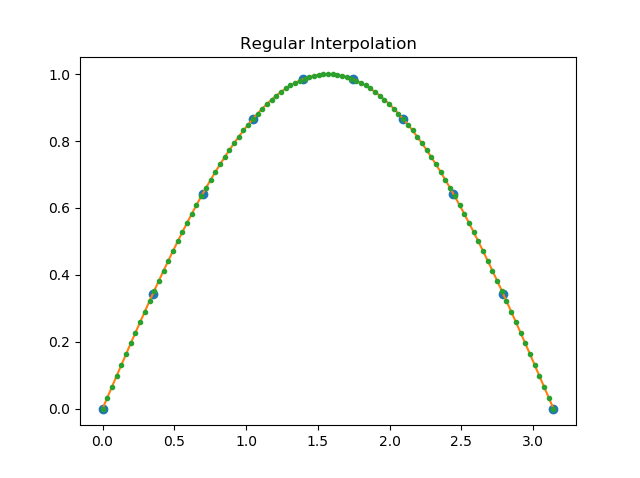
\includegraphics[width=11cm]{regSpline}
\end{center}
\caption{\label{fig:regSpline}Spline interpolation with regularly spaced
points for $\sin(x), x=0,\pi$. The large circles are the data, the dotted
line the exact curve and the orange line the spline curve.}
\end{figure}
Figure~\ref{fig:irregSpline} is the same calculation using irregularly
spaced points.
\begin{figure}
\begin{center}
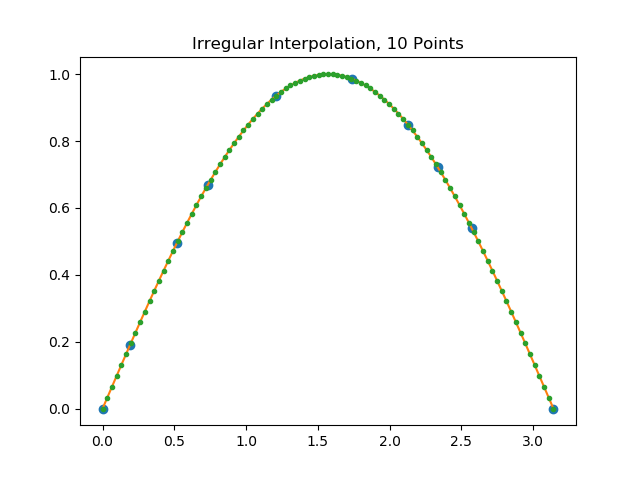
\includegraphics[width=11cm]{irregSpline}
\end{center}
\caption{\label{fig:irregSpline}Spline interpolation with irregularly
spaced points for $\sin(x), x=0,\pi$. The large circles are the data,
the dotted line the exact curve and the orange line the spline curve.}
\end{figure}
Doing the same calculation in Matlab gives similar results.
Figure~\ref{fig:matSpline} is the same calculation done in Matlab
with irregularly spaced points.
\begin{figure}
\begin{center}
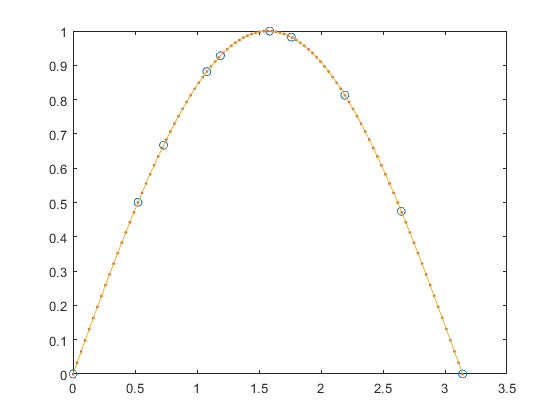
\includegraphics[width=11cm]{matSpline}
\end{center}
\caption{\label{fig:matSpline}Spline interpolation using Matlab
spline routine with irregularly spaced points.
Compare to Figure~\ref{fig:irregSpline}.}
\end{figure}
I also did a range of unit tests on the routine checking for
satisfying the spline equations and for continuity of the function
and its first two derivatives at the knots. All units tests were
passed successfully.

\subsubsection{Extra Oscillations}
If there are jumps in the data making the curve look
discontinuous, a spline can oscillate near the gap.
Consider the data in Figure~\ref{fig:csbump}
\begin{figure}
\begin{center}
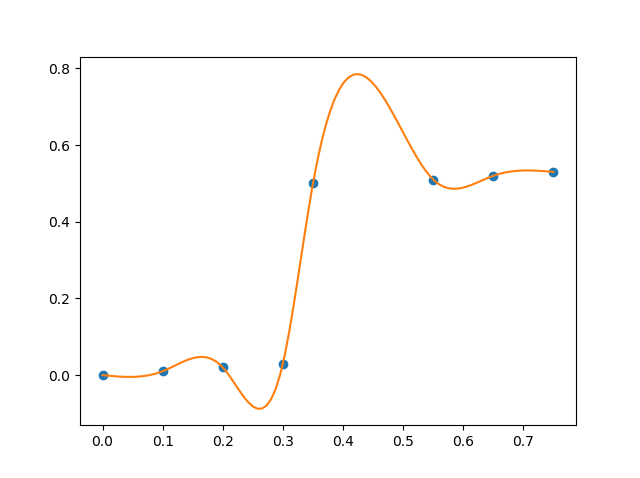
\includegraphics[width=11cm]{csbump}
\end{center}
\caption{\label{fig:csbump}Cubic spline interpolation for
data with a sudden bump.}
\end{figure}
as an example.
In this case, a piece-wise hermite polynomial
may be a better way to go. Matlab
recommends the pchip function\cite{Fritsch,Kahaner} based
on hermite polynomials to address this issue. The spline interpolation
in Matlab is identical to the Julia one. Figure~\ref{fig:pchip}
is what the pchip routine produces.
\begin{figure}
\begin{center}
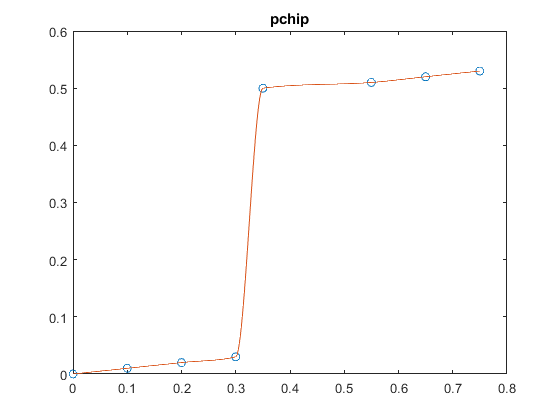
\includegraphics[width=11cm]{pchip}
\end{center}
\caption{\label{fig:pchip}Hermite polynomial interpolation
for data with a sudden bump using pchip in MATLAB.}
\end{figure}

\section{Piece-wise Hermite Polynomials}
I will follow Fritsch's notation\cite{Fritsch}
\begin{align}
f(x) &= y_i H_1(x) + y_{i+1} H_2(x) + d_i H_3(x) + d_{i+1} H_4(x)\\
y_i &= f(x_i)\\
d_i &= f'(x_i)\\
h_i &= x_{i+1}-x{i}\\
H_1(x) &= \phi\left(\frac{x_{i+1}-x}{h_i}\right)\\
H_2(x) &= \phi\left(\frac{x-x_i}{h_i}\right)\\
H_3(x) &= -h_i\psi\left(\frac{x_{i+1}-x}{h_i}\right)\\
H_4(x) &= h_i\psi(\left(\frac{x-x_i}{h_i}\right)\\
\phi(t) &= 3t^2-2t^3\\
\psi(t) &= t^3-t^2
\end{align}
If speed is important, the above nested formulas can undoubtedly
be simplified to make he code more efficient.

The prescription in Fritsch\cite{Fritsch} for producing cubic
hermite interpolants requires the derivatives at the knots. It
is not clear from the documentation which choice the current
version of MATLAB makes in the pchip routine. However, I found
looked through the MATLAB source code to see how this choice
was made.
\subsection{Derivatives}
The formulas in the previous section require the computation of
numerical derivatives at each knot.
\subsubsection{Equally-Spaced Points}
With equally-spaced knots, this
is probably best done using the straightforward "three point formula."
\begin{equation}
y'_i \approx \frac{y_{i+1}-y_{i-1}}{2h},\label{eq:ceq}
\end{equation}
where $h=y_2-y_1=y_3-y_2$.
This formula is accurate to second order in $h$ as can be seen
from a Taylor series expansion of $f(x)$ about the point $x_i$.
\begin{equation}
f(x)=f(x_i)+f'(x_i)(x-x_i)+\frac{1}{2}f''(x_i)(x-x_i)^2+
	\frac{1}{6}f'''(x_i)(x-x_i)^3\label{eq:Taylor}
\end{equation}
Substituting Equation~\ref{eq:Taylor} into Equation~\ref{eq:ceq}
with $y_{i+1}=f(x_i+h)$, $y_{i-1}=f(x_i-h)$ and
$h=x_i-x{i-1}=x_{i+1}-x_i$ yields
\begin{equation}
y'_i=f'(x_i)=f'(x_i)+\frac{1}{6}f'''(x_i)h^2.
\end{equation}
\subsubsection{Unequally-Spaced Points}
If the points are not equally spaced, a somewhat less
accurate formula can be found from the average of the forward
and backward difference formulas.
\begin{align}
f'(x_i) &\approx \frac{f'_b(x_i)+f'_f(x_i)}{2} \label{eq:meanDer}\\
&= \frac{y_i-y_{i-1}}{2h_b}+\frac{y_{i+1}-y_i)}{2h_f}\\
&= \frac{y_{i+1}}{2h_f}+y_i\left(\frac{1}{2h_b}-\frac{1}{2h_f}\right)
	-\frac{y_{i-1}}{2h_b} \label{eq:cuneq}\\
&= \frac{y_{i+1}}{2h_f}+y_i\frac{h_f-h_b}{2h_f h_b}
	-\frac{y_{i-1}}{2h_b}\label{eq:meanb}
\end{align}
where $h_f=y_{i+1}-y{i}$ and $h_b=y_i-y_{i-1}$.
Substituting the Equation~\ref{eq:Taylor} for the terms
in Equation~\ref{eq:cuneq} shows the error in this formula.
\begin{align}
\frac{f(x_{i+1})}{2h_f} &= \frac{f(x_i)}{2h_f}+\frac{f'(x_i)}{2}+
	\frac{1}{4}h_f f''(x_i)+\cdots\\
\frac{f(x_{i-1})}{2h_b} &= \frac{f(x_i)}{2h_b}-\frac{f'(x_i)}{2}+
	\frac{1}{4}h_b f''(x_i)+\cdots\\
\frac{f(x_{i+1})}{2h_f}+f(x_i)\left[\frac{1}{2h_b}-\frac{1}{2h_f}\right]
	-\frac{f(x_{i-1})}{2h_b} &= f'(x_i)+\frac{1}{4}f''(x_i)(h_f-h_b)+\cdots
\end{align}
Thus, the error in this case in linear in $h$ and proportional to
$f''(x_i)$ instead of $f'''(x_i)$ as is the case for equally spaced
points.

Another way to find a derivative is to find the quadratic polynomial
which goes through the three points and take the derivative of that.
Let
\begin{equation}
f(x)=a+b(x-x_i)+c(x-x_i)^2.
\end{equation}
At the point $f(x_{i-1}) = y_{i-1}$
\begin{equation}
y_{i-1} = a-bh_b+ch_b^2.\label{eq:ym}
\end{equation}
At the point $f(x_i)= y_i$
\begin{equation}
y_i = a. \label{eq:yi}
\end{equation}
At the point $f(x_{i+1}) = y_{i+1}$
\begin{equation}
y_{i+1} = a+bh_f+ch_f^2.\label{eq:yp}
\end{equation}
Substituting Equation~\ref{eq:yi} into Equation~\ref{eq:ym}
and Equation~\ref{eq:yi}, solving the remaining equations for $c$
and then equating them to solve for $b$ yields
\begin{equation}
b = f'(x_i) = \frac{(y_i-y_{i-1})h_f}{h_b(h_f+h_b)}+
	\frac{(y_{i+1}-y_i)h_b}{h_f(h_f+h_b)}.\label{eq:quadb}
\end{equation}
Figure~\ref{fig:hermiteBump} compares the cubic Hermite interpolations
using Equation~\ref{eq:meanb} and Equation~\ref{eq:quadb} to the
cubic spline interpolation.
\begin{figure}
\begin{center}
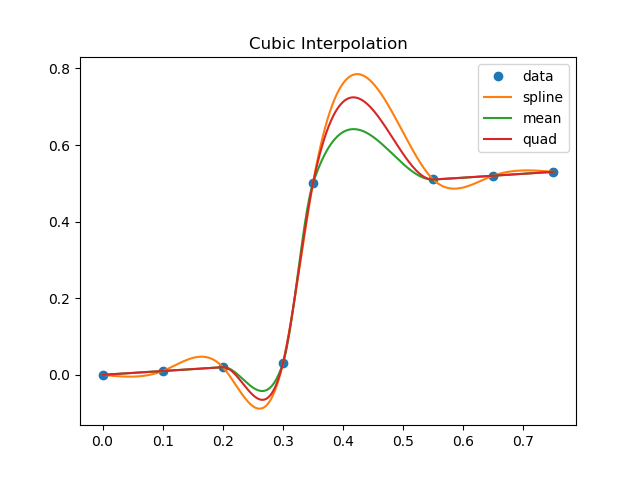
\includegraphics[width=10cm]{hermiteBump}
\end{center}
\caption{\label{fig:hermiteBump}Comparison of spline and hermite
polynomial interpolations for data with a discontinuity. The circles are
the original data points. The curve labeled ``mean''
uses Equation~\ref{eq:meanb}
for the derivatives in the hermite interpolation. The curve labeled
``quad'' uses Equation~\ref{eq:quadb} for the slopes.}
\end{figure}
Note that both choices of slopes still result in overshooting on the
interpolation curve, but not as sever as with the spline. The slope
computed using Equation~\ref{eq:meanb} has less overshoot than the
one computed using Equation~\ref{eq:quadb}.
\subsection{Piece-wise Monotonic Curves}
Fritsch\cite{Fritsch,Wiki} describe a way to make the piece-wise
cubic curve locally monotonic. This should be the same as the pchip
method illustrated in Figure~\ref{fig:pchip}.

The first step is to compute the linear slopes between the data
points.
\begin{align}
\Delta_i &= \frac{y_{i+1}-y_i}{h_i}\\
h_i &= x_{i+1}-x_i
\end{align}
The slopes at the data points are initially chosen to be the average
of the linear slopes (as in Equation~\ref{eq:meanDer}).
\begin{align}
d_i &= \frac{\Delta_{i-1}+\Delta_i}{2}\qquad\mbox{for } i=2,\ldots,n-1\\
d_1 &= \Delta_1\\
d_n &= \Delta_n
\end{align}
If $\Delta_i$ and $\Delta_{i-1}$ have opposite signs, then $d_i=0$.
For $i=1,\ldots,n-1$, if $\Delta_i=0$
\begin{equation}
d_i = d_{i+1}=0
\end{equation}
In this case, the following steps are ignored.
The next step is to define the variables
\begin{align}
\alpha_i &= \frac{d_i}{\Delta_i}\\
\beta_i &= \frac{d_{i+1}}{\Delta i}
\end{align}
The vector $(\alpha_i,\beta_i)$ must have a radius less than 3.
Therefore, if $\alpha_i^2+\beta_i^2>9$,
\begin{align}
\tau_i &= \frac{3}{\sqrt{\alpha_i^2+\beta_i^2}}\\
d_i &= \tau_i \alpha_i \Delta_i\\
d_{i+1} &= \tau_i \beta_i \Delta_i
\end{align}
Figure~\ref{fig:pchipBump} is the interpolation using this algorithm
for the slopes.
\begin{figure}
\begin{center}
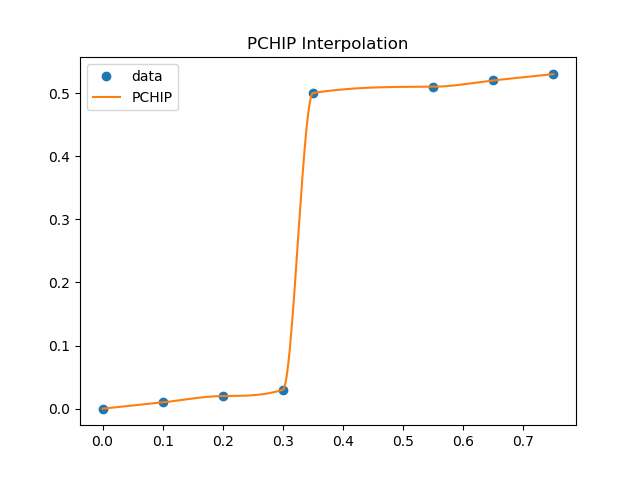
\includegraphics[width=11cm]{pchipBump}
\end{center}
\caption{\label{fig:pchipBump}PCHIP interpolation using my
Julia routine. Compare to the MATLAB calculation in
Figure~\ref{fig:pchip}.}
\end{figure}
\appendix
\section{Spline Solution for Regularly-Spaced Points}\label{sec:reg-deriv}
The goal is to solve Equations~\ref{eq:Yi0} through \ref{eq:Ypi1}
by eliminating the cubic coefficients and only having equations
in terms of the $y_i$ and $D_i$ variables. We first need to
add two more equations.
\begin{align}
Y''_i(0) &= 2c_i\label{eq:ypp0}\\
Y''_i(1) &= Y''_{i+1}(0) = 2c_i+6d_i\label{eq:yppn}\\
c_{i+1} &= c_i + 3d_i. \label{eq:cd}
\end{align}
Substituting in the values for $c_i$ from Equation~\ref{eq:ci} and
$d_i$ from Equation~\ref{eq:di}, Equation~\ref{eq:cd} becomes
\begin{multline}
3(y_{i+2}-y_{i+1})-2D_{i+1}-D_{i+2} = 3(y_{i+1}-y_i)-2D_i-D_{i+1}\\
	+3[2(y_i-y_{i+1})+D_i+D_{i+1}].
\end{multline}
Grouping the $y$ variables on one side of the equation and the $D$
variables on the other,
\begin{equation}
3(y_{i+2}-y_i) = D_{i+2} +4D{i+1} +D_i.
\end{equation}
This accounts for the middle rows of Equation~\ref{eq:eqtd}. The
top and bottom rows come from the initial and final conditions
in Equations~\ref{eq:bslope} and \ref{eq:eslope}. Combining
Equations~\ref{eq:bslope}, \ref{eq:ypp0}, and \ref{eq:ci},
\begin{align}
2c_1 & = 0\\
3(y_2-y_1) &= 2D_1 + D_2,
\end{align}
which is the first row of Equation~\ref{eq:eqtd}. Combining
Equations~\ref{eq:eslope}, \ref{eq:yppn}, \ref{eq:ci}, and
\ref{eq:di},
\begin{align}
2c_n+6d_n &= 0\\
3(y_{n+1}-y_n)-2D_n-D_{n+1}+3[2(y_n-y_{n+1})+D_n+D_{n+1}] &= 0\\
3(y_n-y_{n+1}) &= D_n+2D_{n+1},
\end{align}
which is the bottom row of Equation~\ref{eq:eqtd}.

\section{Spline Solution for Irregularly-Spaced Points}\label{sec:irreg-deriv}
The goal is to solve Equations~\ref{eq:Yi0} through \ref{eq:Ypi1}
by eliminating the cubic coefficients and only having equations
in terms of the $y_i$, $D_i$, and $\alpha_i$ variables.
We first need to add two more equations.
\begin{align}
Y''_i(x_i) &= 2c_i\label{eq:ypp0i}\\
Y''_i(x_{i+1}) &= Y''_{i+1}(x_{i+1})
 = 2c_i+6d_i\alpha_i\label{eq:yppni}\\
c_{i+1} &= c_i + 3d_i \alpha_i. \label{eq:cdi}
\end{align}
Substituting in the values for $c_i$ from Equation~\ref{eq:cirreg} and
$d_i$ from Equation~\ref{eq:dirreg}, Equation~\ref{eq:cdi} becomes
\begin{multline}
3\frac{y_{i+2}-y_{i+1}}{\alpha_{i+1}^2}-2\frac{D_{i+1}}{\alpha_i}
	-\frac{D_{i+2}}{\alpha_{i+1}} = \\
	3\frac{y_{i+1}-y_i}{\alpha_i^2}-2\frac{D_i}{\alpha_i}
	-\frac{D_{i+1}}{\alpha_i}
	+3\left[2\frac{y_i-y_{i+1}}{\alpha_i^2}+\frac{D_i}{\alpha_i}
	+\frac{D_{i+1}}{\alpha_i}\right].
\end{multline}
Grouping the $y$ variables on one side of the equation and the $D$
variables on the other,
\begin{equation}
3\left[\frac{y_{i+2}}{\alpha_{i+1}^2}+y_{i+1}\left(\frac{1}{\alpha_i^2}
	-\frac{1}{\alpha_{i+1}^2}\right)-\frac{y_i}{\alpha_i^2}\right]
	= \frac{D_{i+2}}{\alpha_{i+1}}
		+2D_{i+1}\left(\frac{1}{\alpha_i}+\frac{1}{\alpha_{i+1}}\right)
		+\frac{D_i}{\alpha_i}.
\end{equation}
This accounts for the middle rows of Equation~\ref{eq:eqtdi}. The
top and bottom rows come from the initial and final conditions
in Equations~\ref{eq:bslope} and \ref{eq:eslope}. Combining
Equations~\ref{eq:bslope}, \ref{eq:ypp0i}, and \ref{eq:cirreg},
\begin{align}
2c_1 & = 0\\
3\frac{(y_2-y_1)}{\alpha_1^2} &= 2\frac{D_1}{\alpha_1} + \frac{D_2}{\alpha_1},
\end{align}
which is the first row of Equation~\ref{eq:eqtdi}. Combining
Equations~\ref{eq:eslope}, \ref{eq:yppni}, \ref{eq:cirreg}, and
\ref{eq:dirreg},
\begin{align}
2c_n+6d_n\alpha_n &= 0\\
3\frac{y_{n+1}-y_n}{\alpha_n^2}-2\frac{D_n}{\alpha_n}
	-\frac{D_{n+1}}{\alpha_n}
	+3\left[2\frac{y_n-y_{n+1}}{\alpha_n^2}+\frac{D_n}{\alpha_n}
	+\frac{D_{n+1}}{\alpha_n}\right] &= 0\\
3\frac{y_n-y_{n+1}}{\alpha_n^2} &= \frac{D_n}{\alpha_n}
	+2\frac{D_{n+1}}{\alpha_n},
\end{align}
which is the bottom row of Equation~\ref{eq:eqtd}.

\section{Julia Code}
Here is the Julia 1.0 code I used to do the calculations in this
article. This version has turned off the flags for unit testing
and graphics allow use of the Interp module as a standalone class.
The various units tests and graphical tests illustrate how it
can be used.
\begin{lstlisting}
module Interp
# Code for interpolation for various orders
using LinearAlgebra
using Test
import Base.length

export CubicSpline, interp, slope, slope2, pchip, pchip2, pchip3

unitTests = false
graphicsTests = false
bumpTests = false
# using PyPlot # needed if graphicsTests is true

"""
    CubicSpline(x,a,b,c,d)

concrete type for holding the data needed
    to do a cubic spline interpolation
"""
struct CubicSpline
    x::Union{Array{Float64,1},
        StepRangeLen{Float64,
            Base.TwicePrecision{Float64},
            Base.TwicePrecision{Float64}}}
    a::Array{Float64,1}
    b::Array{Float64,1}
    c::Array{Float64,1}
    d::Array{Float64,1}
end

"""
    PSCHIP(x,a,b,c,d)

concrete type for holding the data needed
    to do a piecewise continuous hermite interpolation
"""
struct PCHIP
    x::Union{Array{Float64,1},
        StepRangeLen{Float64,
            Base.TwicePrecision{Float64},
            Base.TwicePrecision{Float64}}}
    y::Array{Float64,1}
    d::Array{Float64,1}
    h::Array{Float64,1}
end

"""
    CubicSpline(x,y)

Creates the CubicSpline structure needed for cubic spline
interpolation

# Arguments
- `x`: an array of x values at which the function is known
- `y`: an array of y values corresonding to these x values
"""
function CubicSpline(x::Array{Float64,1}, y::Array{Float64,1})
    len = size(x,1)
    if len<3
        error("CubicSpline requires at least three points for interpolation")
    end
    # Pre-allocate and fill columns and diagonals
    yy = zeros(len)
    dl = zeros(len-1)
    du = zeros(len-1)
    dd = zeros(len)
    alpha = x[2:len].-x[1:len-1]
    yy[1] = 3*(y[2]-y[1])/alpha[1]^2
    du[1] = 1/alpha[1]
    dd[1] = 2/alpha[1]
    for i=2:len-1
        yy[i] = 3*(y[i+1]/alpha[i]^2+
            y[i]*(alpha[i-1]^(-2)-alpha[i]^(-2))-
            y[i-1]/alpha[i-1]^2)
        dl[i-1] = 1/alpha[i-1]
        du[i] = 1/alpha[i]
        dd[i] = 2*(1/alpha[i-1]+1/alpha[i])
    end
    yy[len] = 3*(y[len]-y[len-1])/alpha[len-1]^2
    dl[len-1] = 1/alpha[len-1]
    dd[len] = 2/alpha[len-1]
    # Solve the tridiagonal system for the derivatives D
    dm = Tridiagonal(dl,dd,du)
    D = dm\yy
    # fill the arrays of spline coefficients
    a = y[1:len-1]  # silly but makes the code more transparent
    b = D[1:len-1]  # ditto
    c = 3 .*(y[2:len].-y[1:len-1])./alpha[1:len-1].^2 .-
        2*D[1:len-1]./alpha[1:len-1].-D[2:len]./alpha[1:len-1]
    d = 2 .*(y[1:len-1].-y[2:len])./alpha[1:len-1].^3 .+
        D[1:len-1]./alpha[1:len-1].^2 .+
        D[2:len]./alpha[1:len-1].^2
    CubicSpline(x,a,b,c,d)
end

function CubicSpline(x::StepRangeLen{Float64,Base.TwicePrecision{Float64},
	Base.TwicePrecision{Float64}}, y::Array{Float64,1})
	
    len = length(x)
    if len<3
        error("CubicSpline requires at least three points for interpolation")
    end
    # Pre-allocate and fill columns and diagonals
    yy = zeros(len)
    dl = ones(len-1)
    dd = 4.0 .* ones(len)
    dd[1] = 2.0
    dd[len] = 2.0
    yy[1] = 3*(y[2]-y[1])
    for i=2:len-1
        yy[i] = 3*(y[i+1] - y[i-1])
    end
    yy[len] = 3*(y[len]-y[len-1])
    # Solve the tridiagonal system for the derivatives D
    dm = Tridiagonal(dl,dd,dl)
    D = dm\yy
    # fill the arrays of spline coefficients
    a = y[1:len-1]  # silly but makes the code more transparent
    b = D[1:len-1]  # ditto
    c = 3 .*(y[2:len].-y[1:len-1]).-2*D[1:len-1].-D[2:len]
    d = 2 .*(y[1:len-1].-y[2:len]).+D[1:len-1].+D[2:len]
    CubicSpline(x,a,b,c,d)
end

"""
    pchip(x,y)

Creates the PCHIP structure needed for piecewise
    continuous cubic spline interpolation

# Arguments
- `x`: an array of x values at which the function is known
- `y`: an array of y values corresonding to these x values
"""
function pchip(x::Array{Float64,1}, y::Array{Float64,1})
    len = size(x,1)
    if len<3
        error("PCHIP requires at least three points for interpolation")
    end
    h = x[2:len].-x[1:len-1]
    # Pre-allocate and fill columns and diagonals
    d = zeros(len)
    d[1] = (y[2]-y[1])/h[1]
    for i=2:len-1
        d[i] = (y[i+1]/h[i]+y[i]*(1/h[i-1]-1/h[i])-y[i-1]/h[i-1])/2
    end
    d[len] = (y[len]-y[len-1])/h[len-1]
    PCHIP(x,y,d,h)
end

function pchip2(x::Array{Float64,1}, y::Array{Float64,1})
    len = size(x,1)
    if len<3
        error("PCHIP requires at least three points for interpolation")
    end
    h = x[2:len].-x[1:len-1]
    # Pre-allocate and fill columns and diagonals
    d = zeros(len)
    d[1] = (y[2]-y[1])/h[1]
    for i=2:len-1
        d[i] = (y[i]-y[i-1])*h[i]/(h[i-1]*(h[i-1]+h[i])) +
            (y[i+1]-y[i])*h[i-1]/(h[i]*(h[i-1]+h[i]))
    end
    d[len] = (y[len]-y[len-1])/h[len-1]
    PCHIP(x,y,d,h)
end

function pchip3(x::Array{Float64,1}, y::Array{Float64,1})
    len = size(x,1)
    if len<3
        error("PCHIP requires at least three points for interpolation")
    end
    h = x[2:len].-x[1:len-1]
    del = (y[2:len].-y[1:len-1])./h
    # Pre-allocate and fill columns and diagonals
    d = zeros(len)
    d[1] = del[1]
    for i=2:len-1
        if del[i]*del[i-1] < 0
            d[i] = 0
        else
            d[i] = (del[i]+del[i-1])/2
        end
    end
    d[len] = del[len-1]
    for i=1:len-1
        if del[i] == 0
            d[i] = 0
            d[i+1] = 0
        else
            alpha = d[i]/del[i]
            beta = d[i+1]/del[i]
            if alpha^2+beta^2 > 9
                tau = 3/sqrt(alpha^2+beta^2)
                d[i] = tau*alpha*del[i]
                d[i+1] = tau*beta*del[i]
            end
        end
    end
    PCHIP(x,y,d,h)
end

"""
    interp(cs::CubicSpline, v::Float)

Interpolate to the value corresonding to v

# Examples
```
x = cumsum(rand(10))
y = cos.(x);
cs = CubicSpline(x,y)
v = interp(cs, 1.2)
```
"""
function interp(cs::CubicSpline, v::Float64)
    # Find v in the array of x's
    if (v<cs.x[1]) | (v>cs.x[length(cs.x)])
        error("Extrapolation not allowed")
    end
    segment = region(cs.x, v)
    if typeof(cs.x)==Array{Float64,1}
        # irregularly spaced points
        t = v-cs.x[segment]
    else
        # regularly spaced points
        t = (v-cs.x[segment])/(cs.x[segment+1]-cs.x[segment])
    end
    cs.a[segment] + t*(cs.b[segment] + t*(cs.c[segment] +
    	t*cs.d[segment]))
end

function interp(pc::PCHIP, v::Float64)
    if (v<pc.x[1]) | (v>pc.x[length(pc.x)])
        error("Extrapolation not allowed")
    end
    i = region(pc.x, v)
    phi(t) = 3*t^2 - 2*t^3
    psi(t) = t^3 - t^2
    H1(x) = phi((pc.x[i+1]-v)/pc.h[i])
    H2(x) = phi((v-pc.x[i])/pc.h[i])
    H3(x) = -pc.h[i]*psi((pc.x[i+1]-v)/pc.h[i])
    H4(x) = pc.h[i]*psi((v-pc.x[i])/pc.h[i])
    pc.y[i]*H1(v) + pc.y[i+1]*H2(v) + pc.d[i]*H3(v) +
    	pc.d[i+1]*H4(v)
end

"""
    slope(cs::CubicSpline, v::Float)

Derivative at the point corresonding to v

# Examples
```
x = cumsum(rand(10))
y = cos.(x);
cs = CubicSpline(x,y)
v = slope(cs, 1.2)
```
"""
function slope(cs::CubicSpline, v::Float64)
    # Find v in the array of x's
    if (v<cs.x[1]) | (v>cs.x[length(cs.x)])
        error("Extrapolation not allowed")
    end
    segment = region(cs.x, v)
    if typeof(cs.x)==Array{Float64,1}
        # irregularly spaced points
        t = v-cs.x[segment]
    else
        # regularly spaced points
        t = (v-cs.x[segment])/(cs.x[segment+1]-cs.x[segment])
    end
    cs.b[segment] + t*(2*cs.c[segment] + t*3*cs.d[segment])
end

"""
    slope(pc::PCHIP, v::Float)

Derivative at the point corresonding to v

# Examples
```
x = cumsum(rand(10))
y = cos.(x);
pc = pchip(x,y)
v = slope(pc, 1.2)
```
"""
function slope(pc::PCHIP, v::Float64)
    # Find v in the array of x's
    if (v<pc.x[1]) | (v>pc.x[length(pc.x)])
        error("Extrapolation not allowed")
    end
    i = region(pc.x, v)
    phip(t) = 6*t - 6*t^2
    psip(t) = 3*t^2 - 2*t
    H1p(x) = -phip((pc.x[i+1]-v)/pc.h[i])/pc.h[i]
    H2p(x) = phip((v-pc.x[i])/pc.h[i])/pc.h[i]
    H3p(x) = psip((pc.x[i+1]-v)/pc.h[i])
    H4p(x) = psip((v-pc.x[i])/pc.h[i])
    pc.y[i]*H1p(v) + pc.y[i+1]*H2p(v) + pc.d[i]*H3p(v) +
    	pc.d[i+1]*H4p(v)
end

"""
    slope2(cs::CubicSpline, v::Float)

Second derivative at the point corresonding to v

# Examples
```
x = cumsum(rand(10))
y = cos.(x);
cs = CubicSpline(x,y)
v = slope2(cs, 1.2)
```
"""
function slope2(cs::CubicSpline, v::Float64)
    # Find v in the array of x's
    if (v<cs.x[1]) | (v>cs.x[length(cs.x)])
        error("Extrapolation not allowed")
    end
    segment = region(cs.x, v)
    if typeof(cs.x)==Array{Float64,1}
        # irregularly spaced points
        t = v-cs.x[segment]
    else
        # regularly spaced points
        t = (v-cs.x[segment])/(cs.x[segment+1]-cs.x[segment])
    end
    2*cs.c[segment] + 6*t*cs.d[segment]
end

function region(x::Array{Float64,1}, v::Float64)
    # Binary search
    len = size(x,1)
    li = 1
    ui = len
    mi = div(li+ui,2)
    done = false
    while !done
        if v<x[mi]
            ui = mi
            mi = div(li+ui,2)
        elseif v>x[mi+1]
            li = mi
            mi = div(li+ui,2)
        else
            done = true
        end
        if mi == li
            done = true
        end
    end
    mi
end

function region(x::StepRangeLen{Float64,Base.TwicePrecision{Float64},
	Base.TwicePrecision{Float64}}, y::Float64)
    min(trunc(Int,(y-first(x))/step(x)),length(x)-2) + 1
end

function regular_tests()
    @testset "regular interpolation" begin
    # Test not enough points exception
    x = range(1.0, stop=2.0, length=2)
    y = [2.0, 4.0]
    @test_throws ErrorException CubicSpline(x,y)
    x = range(1.0, stop=3.25, length=4)
    y = [1.5, 3.0, 3.7, 2.5]
    cs = CubicSpline(x,y)
    @test_throws ErrorException interp(cs, 0.0)
    @test_throws ErrorException interp(cs, 4.0)
    # Check region
    @test region(x, 1.0) == 1
    @test region(x, 1.2) == 1
    @test region(x, 3.25) == 3
    @test region(x, 2.0) == 2
    @test region(x, 2.8) == 3
    # Check spline at knots
    @test interp(cs, 1.0) == 1.5
    @test interp(cs, 1.75) == 3.0
    @test isapprox(interp(cs, 3.25), 2.5, atol=1e-14)
    # Check spline with unit spacing of knots
    x = range(0.0, stop=4.0, length=5)
    y = sin.(x)
    cs = CubicSpline(x,y)
    dy = cos.(x)
    for i = 1:4
        @test cs.a[i] == y[i]
        @test isapprox(cs.a[i] + cs.b[i] + cs.c[i] +
        	cs.d[i], y[i+1], atol=1.e-12)
        @test isapprox(cs.b[i], dy[i], atol=0.08)
        @test isapprox(cs.b[i] + 2*cs.c[i] + 3*cs.d[i],
        	dy[i+1], atol=0.25)
    end
    end;
end

function irregular_tests()
    x = range(0.0, stop=4.0, length=5)
    y = sin.(x)
    cs = CubicSpline(x,y)
    x = [0.0, 1.0, 2.0, 3.0, 4.0]
    y = sin.(x)
    csi = CubicSpline(x,y)
    @testset "irregular interpolation" begin
    # Test not enough points exception
    x = [1.0, 2.0]
    y = [2.0, 4.0]
    @test_throws ErrorException CubicSpline(x,y)
    x = [0.2, 1.4, 3.8, 5.7]
    y = [1.5, 3.0, 3.7, 2.5]
    csi = CubicSpline(x,y)
    @test_throws ErrorException interp(csi, 0.0)
    @test_throws ErrorException interp(csi, 6.0)
    # Check region
    @test region(x, 0.3) == 1
    @test region(x, 0.2) == 1
    @test region(x, 5.7) == 3
    @test region(x, 2.1) == 2
    @test region(x, 4.0) == 3
    # Check spline at knots
    @test interp(csi, 0.2) == 1.5
    @test interp(csi, 1.4) == 3.0
    @test isapprox(interp(csi, 5.7), 2.5, atol=1e-14)
    # Check spline with unit spacing of knots
    x = [0.0, 1.0, 2.0, 3.0, 4.0]
    y = sin.(x)
    csi = CubicSpline(x,y)
    for i = 1:4
        @test csi.a[i] == cs.a[i]
        @test csi.b[i] == cs.b[i]
        @test csi.c[i] == cs.c[i]
        @test csi.d[i] == cs.d[i]
        @test csi.a[i] == y[i]
        @test isapprox(csi.a[i] + csi.b[i] + csi.c[i] +
        	csi.d[i], y[i+1], atol=1.e-12)
    end
    # Check meeting knot conditions
    for i = 1:3
        di = csi.b[i+1]
        dip = csi.b[i] + 2*csi.c[i] + 3*csi.d[i]
        @test isapprox(di, dip, atol=1.e-12)
    end
    for i = 1:3
        ddi = 2*csi.c[i+1]
        ddip = 2*csi.c[i]+6*csi.d[i]
        @test isapprox(ddi, ddip, atol=1.e-12)
    end
    # Second derivatives at end points
    @test isapprox(csi.c[1], 0.0, atol = 1.e-12)
    @test isapprox(2*csi.c[4]+6*csi.d[4], 0.0, atol = 1.e-12)
    # Test matching boundary conditions with unequally spaced knots
    x = [0.0, 0.7, 2.3, 3.0, 4.1]
    y = sin.(x)
    csi = CubicSpline(x,y)
    for i = 1:4
        @test csi.a[i] == y[i]
        alpha = x[i+1]-x[i]
        yend = csi.a[i] + csi.b[i]*alpha + csi.c[i]*alpha^2
         + csi.d[i]*alpha^3
        # @test isapprox(yend, y[i+1], atol=1.e-12)
    end
    # Check for continuity near knot 2
    eps = 0.0001
    vl = x[2] - eps
    vg = x[2] + eps
    yl = interp(csi, vl)
    yg = interp(csi, vg)
    @test abs(yl-yg) < 2*eps
    sl = slope(csi, vl)
    sg = slope(csi, vg)
    @test abs(sl-sg) < 2*eps
    sl2 = slope2(csi, vl)
    sg2 = slope2(csi, vg)
    @test abs(sl2-sg2) < 2*eps
    # Check meeting knot conditions
    for i = 1:3
        alpha = x[i+1]-x[i]
        dip = csi.b[i+1]
        di = csi.b[i]+2*csi.c[i]*alpha+3*csi.d[i]*alpha^2
        @test isapprox(di, dip, atol=1.e-12)
    end
    for i = 1:3
        alpha = x[i+1]-x[i]
        ddi = 2*csi.c[i+1]
        ddip = 2*csi.c[i]+6*csi.d[i]*alpha
        @test isapprox(ddi, ddip, atol=1.e-12)
    end
    # Second derivatives at end points
    @test isapprox(csi.c[1], 0.0, atol = 1.e-12)
    alpha = x[5] - x[4]
    @test isapprox(2*csi.c[4]+6*csi.d[4]*alpha, 0.0, atol = 1.e-12)
    end;
end

function graphics_tests()
    x = range(0.0, stop=pi, length=10)
    y = sin.(x)
    cs = CubicSpline(x,y)
    xx = range(0.0, stop=pi, length=97)
    yy = [interp(cs,v) for v in xx]
    yyy = sin.(xx)
    figure()
    plot(x,y,"o",xx,yy,"-",xx,yyy,".")
    title("Regular Interpolation")

    x = cumsum(rand(10));
    x = (x.-x[1]).*pi/(x[10].-x[1])
    y = sin.(x)
    cs = CubicSpline(x,y)
    xx = range(0.0, stop=pi, length=97)
    yy = [interp(cs,v) for v in xx]
    yyy = sin.(xx)
    figure()
    plot(x,y,"o",xx,yy,"-",xx,yyy,".")
    title("Irregular Interpolation, 10 Points")
end

function bump_tests()
    x = [0.0, 0.1, 0.2, 0.3, 0.35, 0.55, 0.65, 0.75];
    y = [0.0, 0.01, 0.02, 0.03, 0.5, 0.51, 0.52, 0.53];
    xx = range(0.0,stop=0.75,length=400);
    sp = CubicSpline(x,y);
    yy = [interp(sp, v) for v in xx]
    pc = pchip(x,y)
    yyy = [interp(pc,v) for v in xx]
    pc2 = pchip2(x,y)
    yyy2 = [interp(pc2,v) for v in xx]
    figure()
    plot(x,y,"o",xx,yy,"-",xx,yyy,"-",xx,yyy2,"-")
    title("Cubic Interpolation")
    legend(("data", "spline", "mean","quad"))
    pc3 = pchip3(x,y)
    yyy3 = [interp(pc3,v) for v in xx]
    figure()
    plot(x, y, "o", xx, yyy3, "-")
    title("PCHIP Interpolation")
    legend(("data", "PCHIP"))
end

function regular_pchip_tests()
    @testset "Regular pchip" begin
    end;
end

function irregular_pchip_tests()
    x=[1.0, 1.8, 2.5, 3.0, 3.9];
    y=cos.(x);
    pc=pchip(x,y)
    @testset "Irregular pchip" begin
    for i=1:5
        # Continuity
        @test interp(pc,x[i])==y[i]
    end
    for i = 2:4
        # Continuity of slope
        eps = 0.000001
        @test isapprox(slope(pc,x[i]-eps),slope(pc,x[i]+eps),atol=4*eps)
    end
    end;
end

if unitTests
    regular_tests()
    irregular_tests()
    regular_pchip_tests()
    irregular_pchip_tests()
end

if graphicsTests
    graphics_tests()
end

if bumpTests
    bump_tests()
end

end # module Interp

\end{lstlisting}

\begin{thebibliography}{9}

\bibitem{mathworld}
Weisstein, Eric W. "Cubic Spline." From
\textit{MathWorld}--A Wolfram Web Resource.
\url{http://mathworld.wolfram.com/CubicSpline.html} (accessed
8/17/2018). Citing: Bartels, R. H.; Beatty, J. C.; and Barsky, B. A.
"Hermite and Cubic Spline Interpolation," Ch. 3 in
\textit{An Introduction to Splines for Use in Computer Graphics
and Geometric Modelling}. San Francisco, CA: Morgan Kaufmann,
pp. 9--17, 1998.

\bibitem{Fritsch}
Fritsch, F. N. and R. E. Carlson. "Monotone Piecewise Cubic Interpolation." SIAM Journal on Numerical Analysis. Vol. 17, 1980, pp.238-–246.

\bibitem{Kahaner}
Kahaner, David, Cleve Moler, Stephen Nash. Numerical Methods and Software. Upper Saddle River, NJ: Prentice Hall, 1988.

\bibitem{Wiki}
Wikipedia, "Monotonic cubic interpolation,"
\url{https://en.wikipedia.org/wiki/Monotone\_cubic\_interpolation}
(accessed 23 Aug 2018).

\end{thebibliography}

\end{document}
